\section{RISE}
Similar technology as LIME, uses PyTorch. Newer than LIME, paper asserts to be better.

Original implementation written for PyTorch.

TODO: show masks
TODO: explain the matrix multiplication

\begin{figure}[H]
\centering
\caption{Image from original paper explaining some classes}
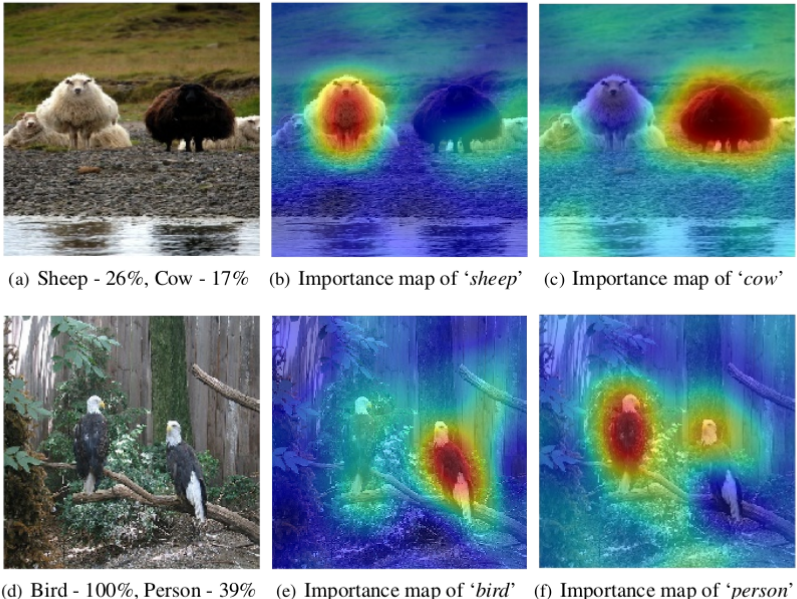
\includegraphics[width=12cm]{chapters/02_methods/images/rise.png}
\end{figure}

\begin{figure}[H]
\centering
\caption{RISE masks}
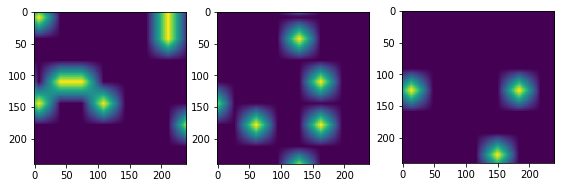
\includegraphics[width=14cm]{chapters/02_methods/images/rise-masks.png}
\end{figure}
